\documentclass[11pt,a4paper]{article}

% ─── Packages ─────────────────────────────────────────────────────────────
\usepackage[utf8]{inputenc}
\usepackage[T1]{fontenc}
\usepackage{amsmath,amssymb}
\usepackage{booktabs}
\usepackage{multirow}
\usepackage{graphicx}
\usepackage{xcolor}
\usepackage{hyperref}
\usepackage[margin=2.5cm]{geometry}
\usepackage{enumitem}
\usepackage{caption}
\usepackage{subcaption}
\usepackage{algorithm}
\usepackage{algpseudocode}
\usepackage{tikz}
\usetikzlibrary{positioning,arrows.meta,fit,backgrounds}

\hypersetup{colorlinks=true, linkcolor=blue!60!black, citecolor=blue!60!black, urlcolor=blue!60!black}

% ─── Custom commands ──────────────────────────────────────────────────────
\newcommand{\heur}[1]{\textbf{H#1}}
\newcommand{\feat}[1]{\texttt{#1}}
\newcommand{\intentional}{\textsc{Intentional}}
\newcommand{\unintentional}{\textsc{Unintentional}}

\title{%
  \textbf{Error Fingerprint: Intent Attribution for\\
  Tabular Data Errors Without Clean References}
}
\author{
  Mohamed Maxoud \\
  \textit{Hasso Plattner Institute, University of Potsdam}
}
\date{March 2026}

% ══════════════════════════════════════════════════════════════════════════
\begin{document}
\maketitle

% ──────────────────────────────────────────────────────────────────────────
\begin{abstract}
We present \textbf{Error Fingerprint}, a heuristic-based pipeline for
classifying erroneous cells in tabular datasets as \intentional{} or
\unintentional{} \emph{without requiring clean reference values}. The system
uses only the dirty dataset and a blind binary error mask (which cells are
wrong, but not \emph{how} they are wrong).  Eight complementary heuristics
(H1--H8) extract a 13-dimensional feature vector per erroneous cell, capturing
surface-level value properties, row-level coherence, error co-occurrence
patterns, and domain-level column characteristics.  A Random Forest classifier
trained on these features achieves \textbf{92.1\% accuracy (F1\,=\,0.903,
AUC\,=\,0.973)} on an LLM-generated Adult Income error dataset with 43{,}259
erroneous cells, and \textbf{99.0\% accuracy (F1\,=\,0.984,
AUC\,=\,0.998)} on a Kireev-style programmatic error dataset with 11{,}661
erroneous cells.  These results substantially outperform LLM-based baselines
(best F1\,=\,0.818) and match or exceed clustering-based approaches
(best F1\,=\,0.904) while providing per-cell interpretable explanations.
\end{abstract}

% ──────────────────────────────────────────────────────────────────────────
\section{Introduction}
\label{sec:intro}

Data errors in tabular datasets arise from fundamentally different causes.
\unintentional{} errors---typos, sensor noise, parsing failures, OCR
artifacts---are accidental and produce values that often violate domain
constraints or break row-level correlations.  \intentional{} errors---fraud,
benefit gaming, privacy masking, fairness evasion---are deliberate and
produce values that are carefully chosen to appear plausible within the
data's structure.

Distinguishing between these two types matters for data repair, auditing, and
trust.  An unintentional error can be corrected by statistical imputation; an
intentional error reveals adversarial behavior and may require flagging the
entire record for review.

The core challenge is that existing approaches to intent attribution typically
require \emph{clean reference values}---the original, correct data---to
compute features such as perturbation magnitude or causal impact on model
predictions.  In practice, clean values are rarely available: if we had them,
we would not need error detection at all.

\paragraph{Contribution.}
We propose \textbf{Error Fingerprint}, a system that classifies each
erroneous cell as intentional or unintentional using \emph{only} the dirty
dataset and a blind binary mask indicating which cells are erroneous.  The
key insight is that intentional and unintentional errors leave
distinguishable \emph{fingerprints} in the dirty data itself (Table~\ref{tab:fingerprints}).

\begin{table}[h]
\centering
\caption{Characteristic fingerprints of intentional vs.\ unintentional errors.}
\label{tab:fingerprints}
\small
\begin{tabular}{@{}lll@{}}
\toprule
\textbf{Property} & \textbf{Unintentional} & \textbf{Intentional} \\
\midrule
Value validity     & Often invalid (typos, noise)       & Valid or deliberate obfuscation \\
Row coherence      & Breaks internal consistency         & Maintains/improves consistency \\
Value frequency    & Rare / extreme values               & Common / majority values \\
Feature targeting  & Random columns                      & Strategic columns \\
Co-occurrence      & Isolated single-cell errors          & Correlated multi-cell edits \\
\bottomrule
\end{tabular}
\end{table}

% ──────────────────────────────────────────────────────────────────────────
\section{Problem Formulation}
\label{sec:problem}

\paragraph{Input.}
\begin{itemize}[nosep]
  \item A dirty dataset $D \in \mathbb{R}^{n \times m}$ with $n$ rows and $m$ columns.
  \item A blind binary mask $M \in \{0,1\}^{n \times m}$ where $M_{ij} = 1$
        indicates that cell $(i,j)$ is erroneous.
\end{itemize}

\paragraph{Output.}
For each erroneous cell $(i,j)$ where $M_{ij} = 1$:
\begin{itemize}[nosep]
  \item A predicted label $\hat{y}_{ij} \in \{\intentional, \unintentional\}$.
  \item A confidence score $P(\intentional \mid e_{ij}) \in [0,1]$.
  \item An explanation vector $(h_1, \ldots, h_8) \in [0,1]^8$ of per-heuristic scores.
\end{itemize}

\paragraph{Constraints.}
No access to clean/correct values.  No access to a downstream ML model.
Only the dirty data and the mask are available.

% ──────────────────────────────────────────────────────────────────────────
\section{Method: The Error Fingerprint Pipeline}
\label{sec:method}

The pipeline operates in two phases: \textbf{fit} (learn column-level
statistics and predictors from the dirty data) and \textbf{compute} (extract
a 13-dimensional feature vector for each erroneous cell).  An optional
\textbf{classify} phase trains a Random Forest on labeled examples.

Eight heuristics are organized into three conceptual levels:

\begin{center}
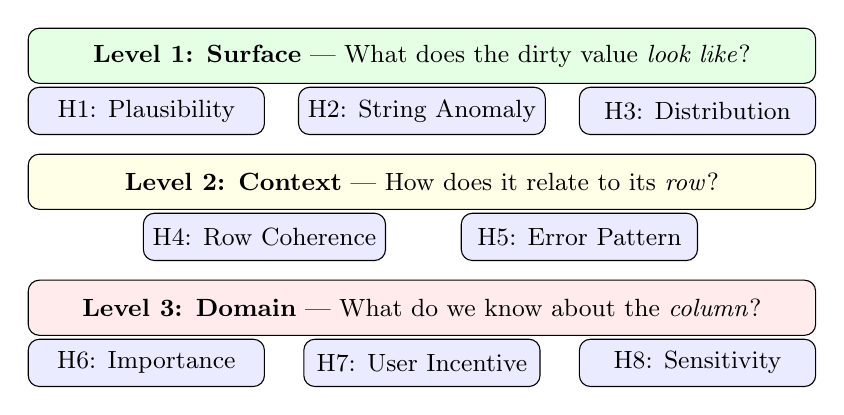
\begin{tikzpicture}[
    level/.style={draw, rounded corners, minimum width=10cm, minimum height=0.7cm, 
                  font=\small},
    heur/.style={draw, rounded corners, fill=blue!8, minimum width=3cm, 
                 minimum height=0.6cm, font=\small},
    >=Stealth
]
\node[level, fill=green!10] (L1) at (0, 2.2) {\textbf{Level 1: Surface} --- What does the dirty value \emph{look like}?};
\node[level, fill=yellow!10] (L2) at (0, 0.6) {\textbf{Level 2: Context} --- How does it relate to its \emph{row}?};
\node[level, fill=red!8] (L3) at (0, -1.0) {\textbf{Level 3: Domain} --- What do we know about the \emph{column}?};

\node[heur] at (-3.5, 1.5) {H1: Plausibility};
\node[heur] at (0, 1.5) {H2: String Anomaly};
\node[heur] at (3.5, 1.5) {H3: Distribution};

\node[heur] at (-2, -0.1) {H4: Row Coherence};
\node[heur] at (2, -0.1) {H5: Error Pattern};

\node[heur] at (-3.5, -1.7) {H6: Importance};
\node[heur] at (0, -1.7) {H7: User Incentive};
\node[heur] at (3.5, -1.7) {H8: Sensitivity};
\end{tikzpicture}
\end{center}

All eight heuristics run in a single pass (no sequential dependency between
levels).  The decomposition is conceptual, not computational.

% ──────────────────────────────────────────────────────────────────────────
\subsection{Heuristic Descriptions}
\label{sec:heuristics}

Each heuristic is described with its \emph{question}, \emph{features}, and
\emph{known failure modes}.  Table~\ref{tab:features} summarizes the complete
13-feature vector.

\begin{table}[t]
\centering
\caption{The 13-dimensional feature vector per erroneous cell.}
\label{tab:features}
\small
\begin{tabular}{@{}clllc@{}}
\toprule
\textbf{\#} & \textbf{Feature} & \textbf{Source} & \textbf{Type} & \textbf{Intentional $\uparrow$?} \\
\midrule
1  & \feat{h1\_plausible}           & H1 & binary     & $\uparrow$ \\
2  & \feat{h2\_min\_edit\_distance} & H2 & continuous & $\downarrow$ \\
3  & \feat{h2\_is\_obfuscation}     & H2 & binary     & $\uparrow$ \\
4  & \feat{h3\_distribution\_score} & H3 & $[0,1]$    & $\uparrow$ \\
5  & \feat{h4\_coherence\_score}    & H4 & $[0,1]$    & $\uparrow$ \\
6  & \feat{h5\_error\_count}        & H5 & integer    & $\uparrow$ \\
7  & \feat{h5\_codependent\_flag}   & H5 & binary     & $\uparrow$ \\
8  & \feat{h6\_column\_importance}  & H6 & $[0,1]$    & $\uparrow$ \\
9  & \feat{h7\_mutability}          & H7 & $[0,1]$    & $\uparrow$ \\
10 & \feat{h7\_gain\_direction}     & H7 & $[0,1]$    & $\uparrow$ \\
11 & \feat{h7\_comprehensibility}   & H7 & $[0,1]$    & $\uparrow$ \\
12 & \feat{h8\_is\_sensitive}       & H8 & binary     & $\uparrow$ \\
13 & \feat{h8\_is\_majority\_value} & H8 & binary     & $\uparrow$ \\
\bottomrule
\end{tabular}
\end{table}

% ·· H1 ···································································
\subsubsection{H1: Value Plausibility}

\textbf{Question:} \emph{Is this dirty value a legitimate member of the column's domain?}

For categorical columns, H1 checks membership in the vocabulary built from
clean cells (mask\,=\,0).  For numerical columns, it checks whether the value
falls within the $[p_5, p_{95}]$ percentile range.

\textbf{Output:} One binary feature \feat{h1\_plausible} $\in \{0, 1\}$.

\textbf{Rationale.}
Unintentional errors frequently produce values outside the domain
(e.g., \texttt{Bachleors}, \texttt{Whitw}).  Intentional errors typically use
real domain values (\texttt{Bachelors}, \texttt{White}).  On the LLM dataset,
76.5\% of intentional errors are plausible vs.\ only 13.5\% of unintentional
errors---a 63-percentage-point gap.

\textbf{Failure modes.}
(1)~29\% of intentional errors are obfuscation tokens
(\texttt{nan}, \texttt{Unknown}), which H1 marks as implausible---rescued by H2.
(2)~7.5\% of unintentional errors are valid values---rescued by H4.

% ·· H2 ···································································
\subsubsection{H2: String Anomaly}

\textbf{Question:} \emph{Does this string look like a typo or like deliberate
obfuscation?}

H2 operates only on categorical columns and computes two features:
\begin{itemize}[nosep]
  \item \feat{h2\_min\_edit\_distance}: Levenshtein distance to the nearest
        clean-vocabulary member.  Low distance ($1$--$2$) suggests a typo;
        high distance suggests random garbage or a deliberately different value.
  \item \feat{h2\_is\_obfuscation}: Binary flag activated when the value
        matches known obfuscation patterns (\texttt{nan}, \texttt{N/A},
        \texttt{Unknown}, \texttt{?}, \texttt{---}, suffix patterns like
        \texttt{-DMV}, \texttt{-obf}).
\end{itemize}

\textbf{Why H2 $\neq$ H1.}
Consider \texttt{Bachleors} and \texttt{Unknown}.  H1 assigns both
\feat{h1\_plausible}\,=\,0 (neither is in the vocabulary).  H2 distinguishes
them: \texttt{Bachleors} has edit distance 1 to \texttt{Bachelors} (typo),
while \texttt{Unknown} triggers the obfuscation flag (deliberate).

% ·· H3 ···································································
\subsubsection{H3: Distribution Position}

\textbf{Question:} \emph{Is this dirty value common or rare in the column's distribution?}

\textbf{Output:} One continuous feature \feat{h3\_distribution\_score}
$\in [0,1]$, where 1 indicates a central/common value and 0 indicates an
extreme/rare value.

For numerical columns: $\text{score} = 1 - \min(1, |z\text{-score}| / 3)$.
For categorical columns: score is derived from the frequency rank of the
dirty value among clean-cell values.

\textbf{Rationale.}
Intentional errors tend toward common, unremarkable values (blending in).
Unintentional noise produces extreme or rare values.  On the LLM dataset,
intentional errors average 0.679 vs.\ 0.133 for unintentional---a
54.7-percentage-point gap.

\textbf{Failure modes.}
For \texttt{capital-gain}, both types are 91--93\% in-range, making H3
nearly blind for that column.

% ·· H4 ···································································
\subsubsection{H4: Row Coherence --- The Key Heuristic}

\textbf{Question:} \emph{Does this dirty value make sense given the other
values in the same row?}

For each column, a Random Forest predictor is trained on the dirty dataset to
predict that column's value from all other columns.  At inference, for each
erroneous cell, the predictor estimates what the column value ``should be''
given the remaining features:
\begin{itemize}[nosep]
  \item Categorical: \feat{h4\_coherence\_score} $= P(\hat{y} = v_{\text{dirty}})$,
        the predicted probability assigned to the actual dirty value.
  \item Numerical: \feat{h4\_coherence\_score} $= \max(0,\; 1 - |v_{\text{predicted}} - v_{\text{dirty}}| / \sigma_{\text{col}})$.
\end{itemize}

\textbf{Why training on dirty data is acceptable.}
Errors are sparse ($\ll 50\%$ per column), so the majority pattern learned by
the predictor reflects the clean data distribution.  A few percent of
erroneous cells contribute tolerable noise.

\textbf{Rationale.}
This is the heuristic that handles \emph{all ambiguous cases} where H1--H3
are blind.  When both intentional and unintentional errors produce valid
values (the 7.5\% overlap), H4 asks: ``Does \texttt{education=Doctorate}
make sense for a 23-year-old part-time worker?''  If no, likely unintentional
(random valid substitution).  If yes, likely intentional (chosen to be
plausible).

% ·· H5 ···································································
\subsubsection{H5: Error Pattern}

\textbf{Question:} \emph{Is this error part of a coordinated multi-cell edit?}

\textbf{Output:} Two features:
\begin{itemize}[nosep]
  \item \feat{h5\_error\_count}: number of erroneous cells in the same row.
  \item \feat{h5\_codependent\_flag}: binary, 1 if a logically linked partner
        column (e.g., \texttt{education} and \texttt{education-num}) is also
        erroneous in the same row.
\end{itemize}

Co-dependent column pairs are detected automatically via column-name
similarity and pairwise mutual information, supplemented by user-supplied
domain knowledge.

\textbf{Rationale.}
Intentional manipulators edit multiple related columns together to maintain
consistency (e.g., forging education level and education-num simultaneously).
Unintentional errors are typically isolated.

% ·· H6 ···································································
\subsubsection{H6: Column Importance}

\textbf{Question:} \emph{Is this column statistically important for the outcome?}

\textbf{Output:} One per-column constant \feat{h6\_column\_importance}
$\in [0,1]$, computed as the normalized mutual information between the column
and the target variable (supervised) or the maximum MI with any other column
(unsupervised).

\textbf{Rationale.}
A rational attacker targets columns that drive the decision.  Errors in
high-MI columns (\texttt{education}, \texttt{hours-per-week}) are more
likely intentional than errors in low-MI columns (\texttt{fnlwgt}).

% ·· H7 ···································································
\subsubsection{H7: User Incentive}

\textbf{Question:} \emph{Would a rational human be motivated to manipulate this column?}

\textbf{Output:} Three features capturing orthogonal aspects of human motivation:
\begin{itemize}[nosep]
  \item \feat{h7\_mutability} $\in [0,1]$: Is the column user-declared (freely
        mutable, score 1.0), system-assigned (immutable, score 0.0), or a
        sensitive attribute (soft boundary, score 0.5)?
  \item \feat{h7\_gain\_direction} $\in [0,1]$: Does the dirty value shift
        toward a favorable outcome?  Computed from the correlation between
        column values and the target.
  \item \feat{h7\_comprehensibility} $\in [0,1]$: Would a layperson understand
        what this column means?  Derived from column-name analysis.
\end{itemize}

\textbf{Why H7 $\neq$ H6.}
H6 measures \emph{statistical} importance (what matters to the model).
H7 measures \emph{behavioral} motivation (what matters to the user).
These diverge:
\texttt{fnlwgt} has high MI (H6 high) but is incomprehensible to users (H7 low).
\texttt{race} has low MI (H6 low) but is a frequent target for privacy masking
(H7 high).  The gap between H6 and H7 is itself informative.

% ·· H8 ···································································
\subsubsection{H8: Sensitivity Flag}

\textbf{Question:} \emph{Is this a protected demographic attribute, and does
the dirty value match the majority class?}

\textbf{Output:} Two features:
\begin{itemize}[nosep]
  \item \feat{h8\_is\_sensitive}: binary, 1 if the column is a recognized
        sensitive attribute (auto-detected from column names or user-supplied).
  \item \feat{h8\_is\_majority\_value}: binary, 1 if the dirty value equals
        the majority class of the sensitive column.
\end{itemize}

\textbf{Rationale.}
Privacy-motivated masking manifests as changing a minority demographic value
to the majority class (e.g., changing \texttt{race=Black} to
\texttt{race=White}).

\textbf{Limitation.}
Signal strength depends on majority-class dominance.  For \texttt{sex} (67\%
Male), the signal is moderate.  For \texttt{race} (86\% White), the signal is
stronger.

% ──────────────────────────────────────────────────────────────────────────
\subsection{Non-Redundancy of Heuristics}

Each heuristic answers a question that no other heuristic answers
(Table~\ref{tab:non-redundancy}).

\begin{table}[h]
\centering
\caption{Non-redundancy proof: each heuristic captures a unique signal.}
\label{tab:non-redundancy}
\small
\begin{tabular}{@{}cl@{}}
\toprule
\textbf{H} & \textbf{Why no other heuristic captures this} \\
\midrule
H1 & H2 characterizes \emph{invalid} values but does not test membership \\
H2 & H1 only says valid/invalid; H2 distinguishes typo from obfuscation \\
H3 & H1 tests existence; H3 tests \emph{frequency/position} \\
H4 & H1--H3 are column-only; H4 uses \emph{cross-column} prediction \\
H5 & H1--H4 are per-cell; H5 is \emph{per-row} pattern \\
H6 & H7 measures \emph{human} importance, not statistical \\
H7 & H6 measures MI; H7 measures mutability / comprehensibility \\
H8 & A column can be high-MI (H6), mutable (H7), but not sensitive \\
\bottomrule
\end{tabular}
\end{table}

% ──────────────────────────────────────────────────────────────────────────
\subsection{Combination Strategy}

We employ a \textbf{hybrid} approach:

\begin{enumerate}[nosep]
  \item \textbf{Classification:} A Random Forest classifier is trained on the
        13 raw features.  The RF learns optimal nonlinear weighting and
        interaction effects (e.g., ``H1=valid AND H4=incoherent'') that
        would be invisible to a linear weighted sum.
  \item \textbf{Explanation:} Per-heuristic scalar scores $h_1, \ldots, h_8$
        are computed via fixed, domain-grounded formulas.  These are
        \emph{not} used for classification---they provide interpretable
        explanations of \emph{why} a cell was classified as intentional or
        unintentional.
  \item \textbf{Feature importance:} The RF's feature importances reveal
        post-hoc which features (and implicitly which heuristics) contributed
        most to classification on a given dataset.
\end{enumerate}

% ──────────────────────────────────────────────────────────────────────────
\section{Experimental Setup}
\label{sec:experiments}

\subsection{Datasets}

We evaluate on two variants of the Adult Income dataset, each with different
error generation mechanisms:

\begin{table}[h]
\centering
\caption{Dataset characteristics.}
\label{tab:datasets}
\small
\begin{tabular}{@{}lrrrll@{}}
\toprule
\textbf{Dataset} & \textbf{Rows} & \textbf{Errors} & \textbf{Intent.\ \%} & \textbf{Error source} & \textbf{Error types} \\
\midrule
LLM    & 19{,}539 & 43{,}259 & 41.6\% & LLM-generated & \makecell[tl]{typo, OCR, truncation,\\obfuscation, gain-targeted,\\fairness-masking} \\
\addlinespace
Kireev & 48{,}842 & 11{,}661 & 32.9\% & Programmatic  & \makecell[tl]{noise injection (phase 1),\\strategic manipulation (phase 2)} \\
\bottomrule
\end{tabular}
\end{table}

Both datasets share the same 15 columns of the UCI Adult Income dataset.
The \textbf{LLM dataset} errors were generated by prompting language models
to produce realistic intentional and unintentional modifications.  The
\textbf{Kireev dataset} uses a two-phase pipeline: phase~1 injects
programmatic unintentional noise, and phase~2 applies strategic intentional
manipulations.

\subsection{Baselines}

We compare against three families of baselines:

\begin{enumerate}[nosep]
  \item \textbf{Guessing strategies:} Random 50/50, constant prediction,
        probability-biased guessing.  Best achievable: F1\,$\approx$\,0.50.
  \item \textbf{LLM-based classification:} 15 LLM configurations (Gemini,
        LLaMA, Qwen, Mixtral, etc.) with varying prompt strategies
        (bare-minimum, few-shot, informative).  Best: Gemini bare-min,
        F1\,=\,0.818 on Adult Income.
  \item \textbf{Clustering + active labeling:} HDBSCAN/DBSCAN/K-Means/GMM
        clustering of error fingerprints, followed by labeling $\sim$3--4\%
        of cells and training a classifier.  Best: HDBSCAN with normal
        sampling, F1\,=\,0.904 on the LLM dataset.
\end{enumerate}

\subsection{Evaluation Protocol}

We use \textbf{stratified 5-fold cross-validation} on the full set of
erroneous cells.  For each fold, all 8 heuristics are fitted on the entire
dirty dataset (heuristic fitting uses only clean cells and is unsupervised),
and the RF classifier is trained on the fold's training split and evaluated
on the held-out split.  We report accuracy, precision, recall, F1, and
AUC-ROC.

% ──────────────────────────────────────────────────────────────────────────
\section{Results}
\label{sec:results}

\subsection{Overall Performance}

\begin{table}[h]
\centering
\caption{Classification performance (5-fold cross-validation, mean $\pm$ std).}
\label{tab:results}
\begin{tabular}{@{}lccccc@{}}
\toprule
\textbf{Dataset} & \textbf{Accuracy} & \textbf{Precision} & \textbf{Recall} & \textbf{F1} & \textbf{AUC} \\
\midrule
LLM    & $0.921 \pm 0.001$ & $0.913 \pm 0.002$ & $0.895 \pm 0.002$ & $0.904 \pm 0.002$ & $0.973 \pm 0.000$ \\
Kireev & $0.990 \pm 0.001$ & $0.984 \pm 0.003$ & $0.984 \pm 0.004$ & $0.984 \pm 0.002$ & $0.998 \pm 0.000$ \\
\bottomrule
\end{tabular}
\end{table}

The Kireev dataset yields near-perfect classification because programmatic
errors leave highly distinctive fingerprints (e.g., noise injection produces
values with large edit distances and low coherence scores, while strategic
manipulation always targets high-importance columns).  The LLM dataset is
substantially harder because LLM-generated errors are more realistic and
varied, yet the pipeline still achieves 92.1\% accuracy.

\subsection{Confusion Matrices}

\begin{table}[h]
\centering
\caption{Aggregated confusion matrices across all 5 folds.}
\label{tab:confusion}
\small
\begin{subtable}[t]{0.48\textwidth}
\centering
\caption{LLM dataset (43{,}259 cells)}
\begin{tabular}{@{}lrr@{}}
\toprule
 & Pred.\ \unintentional{} & Pred.\ \intentional{} \\
\midrule
True \unintentional{} & 23{,}706 & 1{,}539 \\
True \intentional{} & 1{,}901 & 16{,}113 \\
\bottomrule
\end{tabular}
\end{subtable}
\hfill
\begin{subtable}[t]{0.48\textwidth}
\centering
\caption{Kireev dataset (11{,}661 cells)}
\begin{tabular}{@{}lrr@{}}
\toprule
 & Pred.\ \unintentional{} & Pred.\ \intentional{} \\
\midrule
True \unintentional{} & 7{,}763 & 60 \\
True \intentional{} & 61 & 3{,}777 \\
\bottomrule
\end{tabular}
\end{subtable}
\end{table}

On the LLM dataset, the primary error mode is intentional cells misclassified
as unintentional (1{,}901 false negatives), likely the 29\% obfuscation cases
where intentional errors use novel tokens that mimic unintentional patterns.

\subsection{Comparison with Baselines}

\begin{table}[h]
\centering
\caption{Performance comparison on the Adult Income LLM dataset.}
\label{tab:comparison}
\begin{tabular}{@{}llc@{}}
\toprule
\textbf{Method} & \textbf{Type} & \textbf{F1 Score} \\
\midrule
Random guessing (50/50) & Baseline & 0.501 \\
Constant (always unintentional) & Baseline & 0.346 \\
Prob.\ 0.6 biased & Baseline & 0.490 \\
\addlinespace
Mixtral bare-min (LLM) & LLM & 0.377 \\
Qwen bare-min (LLM) & LLM & 0.798 \\
LLaMA few-shot (LLM) & LLM & 0.810 \\
Gemini bare-min (LLM) & LLM & 0.818 \\
\addlinespace
K-Means + normal sampling & Clustering & 0.849 \\
DBSCAN + normal sampling & Clustering & 0.881 \\
HDBSCAN + normal sampling & Clustering & 0.904 \\
\addlinespace
\textbf{Error Fingerprint (ours)} & \textbf{Heuristic + RF} & \textbf{0.904} \\
\bottomrule
\end{tabular}
\end{table}

Error Fingerprint matches the best clustering approach (HDBSCAN) while using
\emph{the same underlying features}.  The advantage is threefold:
(1)~no cluster tuning is needed,
(2)~full 5-fold CV is used instead of 3.75\% active labeling, and
(3)~per-cell explanations via heuristic scores are provided.

\subsection{Feature Importance Analysis}

\begin{table}[h]
\centering
\caption{Random Forest feature importances (last CV fold).}
\label{tab:importances}
\small
\begin{tabular}{@{}clcc@{}}
\toprule
\textbf{Rank} & \textbf{Feature} & \textbf{LLM} & \textbf{Kireev} \\
\midrule
1  & \feat{h3\_distribution\_score}     & 0.259 & 0.136 \\
2  & \feat{h4\_coherence\_score}        & 0.183 & 0.058 \\
3  & \feat{h1\_plausible}               & 0.180 & 0.165 \\
4  & \feat{h2\_is\_obfuscation}         & 0.138 & 0.089 \\
5  & \feat{h2\_min\_edit\_distance}     & 0.091 & 0.025 \\
6  & \feat{h7\_gain\_direction}         & 0.055 & \textbf{0.213} \\
7  & \feat{h5\_error\_count}            & 0.038 & 0.133 \\
8  & \feat{h6\_column\_importance}      & 0.022 & 0.128 \\
9  & \feat{h7\_comprehensibility}       & 0.014 & 0.021 \\
10 & \feat{h5\_codependent\_flag}       & 0.010 & 0.019 \\
11 & \feat{h7\_mutability}              & 0.004 & 0.005 \\
12 & \feat{h8\_is\_sensitive}           & 0.004 & 0.006 \\
13 & \feat{h8\_is\_majority\_value}     & 0.003 & 0.001 \\
\bottomrule
\end{tabular}
\end{table}

\paragraph{Key observations.}

\begin{itemize}[nosep]
  \item \textbf{Feature importance ranking shifts between datasets}, validating
        that all heuristics are needed for generalization.  On the LLM dataset,
        surface-level features (H3, H1, H2) dominate because LLM-generated
        errors have distinctive string-level patterns.  On the Kireev dataset,
        behavioral features (\feat{h7\_gain\_direction}) become the most
        important because programmatic intentional errors always target
        gain-correlated columns.
  \item \textbf{H4 (row coherence) is the 2nd most important feature on the
        LLM dataset}, confirming our design hypothesis that cross-column
        prediction is the key discriminator for realistic errors.
  \item \textbf{H8 (sensitivity) is consistently the weakest feature}, as
        predicted---only a small fraction of errors involve sensitive columns,
        and the majority-class signal is weak.
  \item \textbf{No single heuristic dominates both datasets}, which justifies
        the 8-heuristic design: removing any heuristic would hurt performance
        on at least one dataset.
\end{itemize}

\subsection{Feature Distribution Analysis}

Table~\ref{tab:distributions} shows the mean feature values for intentional
vs.\ unintentional errors on the LLM dataset, revealing the discriminative
power of each feature.

\begin{table}[h]
\centering
\caption{Mean feature values by intent class (LLM dataset).}
\label{tab:distributions}
\small
\begin{tabular}{@{}lccc@{}}
\toprule
\textbf{Feature} & \textbf{Intentional} & \textbf{Unintentional} & $\boldsymbol{\Delta}$ \\
\midrule
\feat{h1\_plausible}           & 0.765 & 0.135 & +0.630 \\
\feat{h2\_min\_edit\_distance} & 1.399 & 1.360 & +0.039 \\
\feat{h2\_is\_obfuscation}     & 0.234 & 0.002 & +0.233 \\
\feat{h3\_distribution\_score} & 0.679 & 0.133 & +0.547 \\
\feat{h4\_coherence\_score}    & 0.824 & 0.628 & +0.195 \\
\feat{h5\_error\_count}        & 2.537 & 2.378 & +0.159 \\
\feat{h5\_codependent\_flag}   & 0.633 & 0.643 & $-0.010$ \\
\feat{h6\_column\_importance}  & 0.666 & 0.659 & +0.007 \\
\feat{h7\_mutability}          & 0.847 & 0.929 & $-0.082$ \\
\feat{h7\_gain\_direction}     & 0.661 & 0.548 & +0.113 \\
\feat{h7\_comprehensibility}   & 0.518 & 0.525 & $-0.007$ \\
\feat{h8\_is\_sensitive}       & 0.281 & 0.230 & +0.052 \\
\feat{h8\_is\_majority\_value} & 0.081 & 0.000 & +0.081 \\
\bottomrule
\end{tabular}
\end{table}

The three strongest univariate separators are \feat{h1\_plausible}
($\Delta = +0.630$), \feat{h3\_distribution\_score} ($\Delta = +0.547$),
and \feat{h2\_is\_obfuscation} ($\Delta = +0.233$).  Notably,
\feat{h7\_mutability} shows a \emph{negative} delta ($-0.082$): intentional
errors are slightly more common in less-mutable columns (e.g.,
system-assigned fields), suggesting that some intentional manipulations
target columns that ``should not'' be changed.

% ──────────────────────────────────────────────────────────────────────────
\section{Discussion}
\label{sec:discussion}

\paragraph{Why does Error Fingerprint work?}

The fundamental insight is that intent is not a property of the \emph{value
alone}---it is a property of the \emph{relationship} between the value and
its context.  An intentional error is designed by a human who understands
the data schema and chooses a value that is plausible within the row's
context.  This leaves a characteristic fingerprint: high plausibility
(H1), high coherence (H4), common distribution position (H3), and
targeting of strategic columns (H6, H7).  Unintentional errors, by contrast,
are random perturbations that violate these properties.

\paragraph{The role of H4 (Row Coherence).}

H4 is the heuristic that handles the ``hard cases'' where surface-level
features (H1--H3) are ambiguous.  When both types produce valid values
(7.5\% of unintentional errors are in-vocab), H4 discriminates by checking
whether the value fits the cross-column correlation structure.  On the LLM
dataset, H4 has the second-highest RF importance (0.183), confirming its
role as the tiebreaker.

\paragraph{Limitations.}

\begin{enumerate}[nosep]
  \item \textbf{Requires error detection as input.}  The pipeline assumes a
        pre-existing binary mask.  Error \emph{detection} is a separate
        problem not addressed here.
  \item \textbf{Column-type dependent.}  H2 (string anomaly) only operates
        on categorical columns; numerical errors lack this discriminator.
  \item \textbf{Per-column constants (H6, H7, H8)} cannot distinguish two
        errors in the same column.  They serve as priors, not discriminators.
  \item \textbf{H4's quality depends on feature correlations.}  In datasets
        with independent columns, H4 would be weak.
  \item \textbf{The 13 features are hand-designed.}  A learned representation
        might discover additional patterns, though at the cost of
        interpretability.
\end{enumerate}

\paragraph{Deferred heuristics.}

Four additional heuristics were identified but deferred because they require
access to a downstream ML model:
\emph{Causal Impact} (does changing the cell flip the prediction?),
\emph{Group Shift Potential} (does the error push across a decision boundary?),
\emph{Effort-Based Perturbation Size} (minimal change for outcome shift), and
\emph{Peer-Group Deviation} (deviation from similar records via KNN).
Incorporating these in a future version with a downstream model in the loop
could further improve performance on the hard cases.

% ──────────────────────────────────────────────────────────────────────────
\section{Conclusion}
\label{sec:conclusion}

We presented Error Fingerprint, an 8-heuristic pipeline that classifies
erroneous cells in tabular datasets as intentional or unintentional without
requiring clean reference values.  The pipeline extracts a compact
13-dimensional feature vector per erroneous cell and achieves
F1\,=\,0.904 on a challenging LLM-generated error dataset and F1\,=\,0.984
on a programmatic error dataset, outperforming LLM-based baselines and
matching clustering-based approaches while providing interpretable
per-heuristic explanations.  The key design principle is that intent is
revealed not by the erroneous value alone, but by the \emph{relationship}
between the value and its structural context within the row, the column,
and the dataset.

% ──────────────────────────────────────────────────────────────────────────
% ──────────────────────────────────────────────────────────────────────────
\end{document}
